%! TEX root = ../main.tex
\documentclass[main]{subfiles}

\begin{document}
    \chapter{路線バス運行スケジュール最適化問題}
    \section{問題概要}
    本研究では,現在の長野市の公共交通システムのモデリングを行い,移動者の移動時間短縮とバスの乗車率向上を目的とした,路線バスの運行スケジュールの最適化を行う.
    解候補は,各路線バスの発車間隔を5の倍数の整数値で表現する.また,本研究において最適化を行う上で交通流シミュレータを用いる.
    交通シミュレータに必要なデータを入力し,シミュレーションを行う.
    その出力結果を元車両と歩行者の総移動時間及びバス乗車率を算出し,解の評価関数の計算を行う.
    上記で述べた最適化のプロセスは図\ref{algo}に示す.
    計画リストをシミュレーションし,その評価値を評価値リストに格納する.
    この評価値リストをもとに,遺伝的アルゴリズムを用いた最適化を行い運行スケジュールを更新する.
    この処理を反復することで最適な運行スケジュールを導出する.
    \begin{figure}
        \centering
        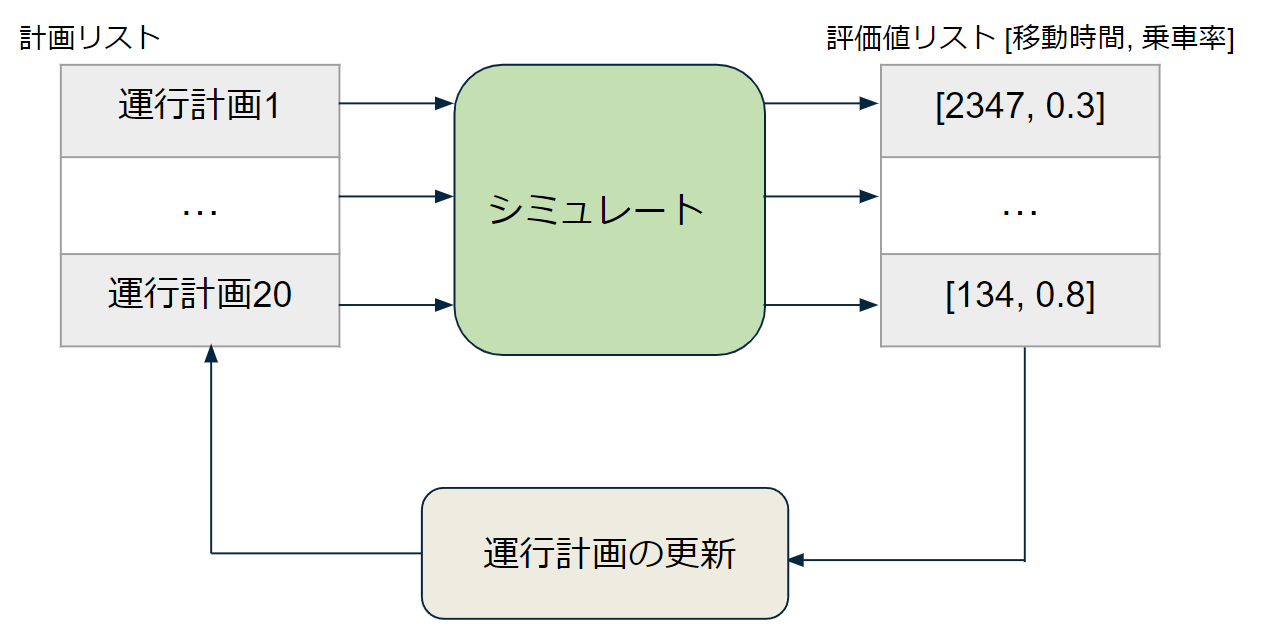
\includegraphics[width=\linewidth]{figures/algo.png}
        \caption{最適化のプロセス}
        \label{algo}
    \end{figure}

    \section{交通流シミュレータ}
        \subsection{概要}
        本研究では,ドイツ航空宇宙センター (DLR) によって開発されたオープンソースの
        交通流シミュレータSUMO(Simulation of Urban Mobility)\cite{sumo}をシミュレータとして用いる.
        オープンストリートマップ形式からSUMO形式に簡単に変換できるため交通ネットワークの構築が容易にできることが特徴のひとつである.
        本研究ではオープンストリートマップから交通ネットワークを作成し,
        NETDITという視覚的なネットワークエディタを使い,より現実に近い状況を作りシミュレートを行う.
        \subsection{SUMOの動作}
        本研究では,オープンストリートマップから交通ネットワークを読み込み,ランダムで交通需要を構成しシミュレートする.
        シミュレーションの入力値としては,道や交差点,信号,建物などのネットワークに関する情報,自
        動車や歩行者、バス停、運行時刻などの情報を用いる.
        移動者に関する情報としては,車両のタイプ,出発地点となる地点の番号と出発地点を出発する時刻,目的地の地点の番号,ルートなどの情報を用いる.
        SUMOは入力された情報をもとにシミュレートを行い,車両の排気ガス排出量,到着までにかかった時間など求めることが出来る.
        SUMOでは,入力ファイルはxml形式で記述する.
        本研究では,路線バスの各路線ごとの発車間隔を変えてシミュレートを行う.
        1回のシミュレートが終わるごとに,交通状況に関する情報が記載されたoutput.txtを出力する.
    
    \section{シミュレート環境の設定}
    本研究では,先行研究\cite{senkoukenkyu}と同じ設定でシミュレートを行う.
    よって,移動者の設定や最適化するバス路線,シミュレートする時間,シミュレートする範囲は
    先行研究\cite{senkoukenkyu}の2.3.2 SUMOの動作について と 2.4 最適化を行うテストモデル を参照されたい.
    
    \section{遺伝子設計}
    バス路線の発車間隔を遺伝子で表現する必要がある.
    各路線は上りと下りの2方向があるため,遺伝子の長さは最適化するバス路線数の2倍となる.
    本研究では,5つのバス路線を最適化するため,遺伝子の長さは10となる.
    各バス路線ごとに,上りと下りの発車間隔を順に並べ一つの配列として,これを遺伝子とする.
    
    \section{評価関数}
    本研究では,路線バス運行スケジュールの評価をするために,2つの評価関数を用いる.
    この2つの評価関数を多目的最適化として解く.
    
        \subsection{総移動時間}
        総移動時間を式\ref{sd}で表す.
        \begin{equation}
            f_1 = \sum_{i=1}^{k} B_i + \sum_{i=1}^{l} V_i
            \label{sd}
        \end{equation}
        $B_i$は各バス利用者の移動時間,$V_i$は各車両の移動時間,kとlはそれぞれバス利用者数と車両数を表す.
        これにより$f_1$は歩行者と車両の総移動時間を表す.
        \subsection{乗車率}
        乗車率を式\ref{zyo}で表す.
        \begin{equation}
            f_2 = \frac{1}{TC} \sum_{i=1}^{T} \frac{n_i}{r_i}
            \label{zyo}
        \end{equation}
        $T$はシミュレーション時間,$C$はバス1台あたりの定員数, $n_i$はシミュレーション開始時から$i$秒目のバスの乗客数,
        $r_i$はシミュレーション開始時から$i$秒目の走行中のバスの台数を示す.
        これにより,$f_2$は1秒あたりの乗車率の平均を表す.
\end{document}